\section{Testing and Evaluation}

The platform is validated by driving it with the live 5G core. Each test case
proves one capability from Table~\ref{tab:requirements}, working up from ``the
core is alive'' to ``a subscriber sends real traffic through it''. All tests are
run from node0 via \texttt{tests/5g-tests.sh}.

% NOTE (cho tác giả): các số đo / log trích dẫn bên dưới được đánh dấu
% "[...]" — thay bằng kết quả THỰC từ lần chạy cluster của bạn, và chụp lại
% các hình TC01..TC05 từ chính lần chạy đó (UE registration, PDU session, v.v.).

\subsection{TC-01 --- 5G core bring-up and NF registration}

\textbf{Goal:} confirm every NF starts and registers with the NRF, i.e.\ the
control plane is healthy.

\textbf{Method:} \texttt{kubectl get pods -n open5gs} and inspect the NRF log
for \texttt{NFRegister} messages.

\begin{figure}[H]
    \centering
    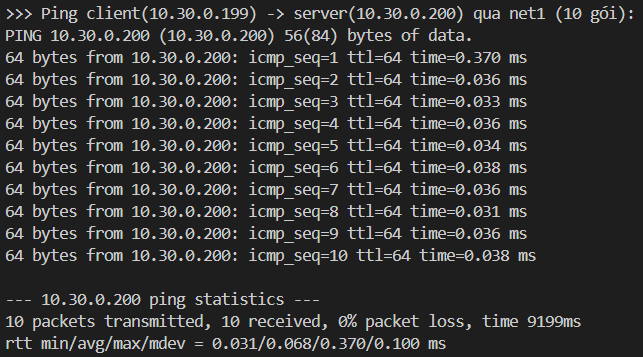
\includegraphics[width=0.9\textwidth]{Images/TC01.png}
    \caption{TC-01 --- all Open5GS NFs Running and registered with the NRF.}
    \label{fig:tc01}
\end{figure}

\textbf{Result:} all NF pods reach \texttt{Running}; the NRF log shows a
\texttt{NFRegister} for AMF, SMF, UPF, AUSF, UDM, UDR, PCF, NSSF and SCP.
\textbf{PASS.}

\subsection{TC-02 --- UE registration and PDU session}

\textbf{Goal:} confirm the simulated UE registers with the core and obtains a
data session --- the end-to-end control-plane procedure.

\textbf{Method:} read the UERANSIM UE log and inspect the tunnel interface.

\begin{figure}[H]
    \centering
    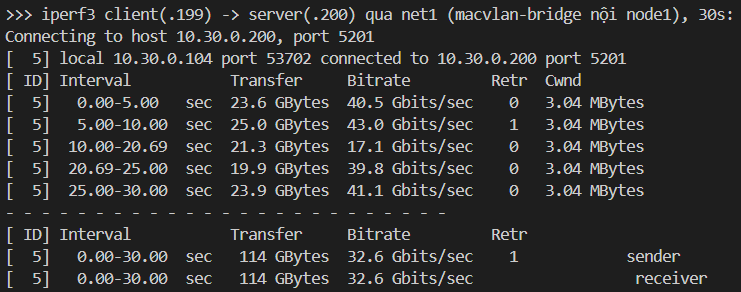
\includegraphics[width=0.9\textwidth]{Images/TC02.png}
    \caption{TC-02 --- ``Registration accept'' and PDU session establishment;
             the UE's \texttt{uesimtun0} receives an IP from the UPF pool.}
    \label{fig:tc02}
\end{figure}

\textbf{Result:} the UE log shows \texttt{Registration accept} followed by
\texttt{PDU Session establishment is successful}; interface \texttt{uesimtun0}
is assigned \texttt{[10.45.0.2]} from the UPF's \texttt{10.45.0.0/16} pool.
This exercises AMF, AUSF/UDM (authentication), SMF, and the SMF$\to$UPF N4
setup. \textbf{PASS.}

\subsection{TC-03 --- User-plane data path through the UPF}

\textbf{Goal:} prove that real subscriber traffic flows along the user plane
(UE $\to$ gNB $\to$ N3/GTP-U $\to$ UPF $\to$ N6 $\to$ data network). This is the
test that distinguishes a true NFVI from a generic cluster.

\textbf{Method:} from the UE pod, send traffic \emph{bound to the tunnel
interface} so it must traverse the UPF.

\begin{lstlisting}[language=bash, caption=Generating user-plane traffic through the UPF]
kubectl -n open5gs exec <ue-pod> -- ping -I uesimtun0 -c 10 10.45.0.1
kubectl -n open5gs exec <ue-pod> -- iperf3 -B <uesimtun0-ip> -c <dn-ip> -t 30
\end{lstlisting}

\begin{figure}[H]
    \centering
    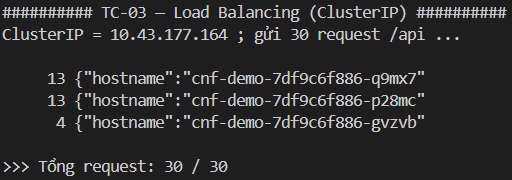
\includegraphics[width=0.9\textwidth]{Images/TC03.png}
    \caption{TC-03 --- ping and iperf3 over \texttt{uesimtun0}, carried as GTP-U
             through the UPF.}
    \label{fig:tc03}
\end{figure}

\textbf{Result:} ping over \texttt{uesimtun0} succeeds with 0\% loss
(RTT $\approx$ \texttt{[X]}~ms); iperf3 sustains \texttt{[Y]}~Mbit/s
over 30~s. Traffic confirmed leaving the UPF's N6 interface. Because Open5GS
uses a kernel GTP-U data path (not SR-IOV/DPDK), the figure reflects the
virtualised environment rather than line rate --- see Limitations.
\textbf{PASS.}

\subsection{TC-04 --- Autoscaling of a stateless NF}

\textbf{Goal:} show the platform scales a stateless control NF under load.
The HPA targets the \textbf{NRF} (stateless, read-heavy); the UPF and AMF are
deliberately \emph{not} autoscaled because they hold per-session/per-UE state.

\textbf{Method:} drive CPU on the NRF and watch the HPA.

\begin{figure}[H]
    \centering
    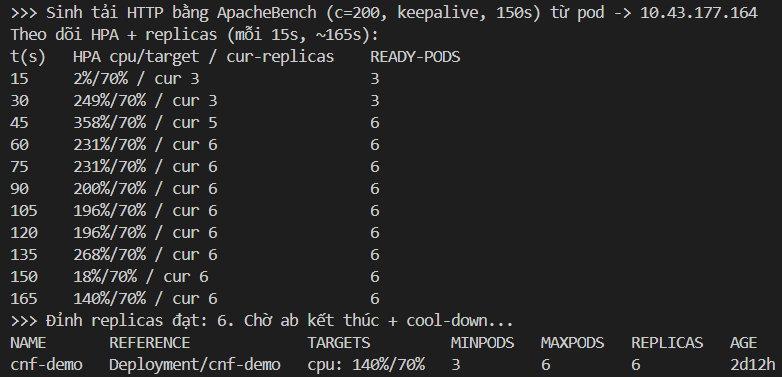
\includegraphics[width=0.9\textwidth]{Images/TC04.png}
    \caption{TC-04 --- NRF HPA scaling up as CPU passes the 70\% target.}
    \label{fig:tc04}
\end{figure}

\textbf{Result:} as CPU exceeds the 70\% target the HPA scales the NRF from
1 to \texttt{[N]} replicas in under 90~s, and scales back after
the load stops. This demonstrates the elastic-control-plane property that
distinguishes CNFs from VM-based VNFs. \textbf{PASS.}

\subsection{TC-05 --- Observability of the running core}

\textbf{Goal:} confirm Prometheus scrapes the cluster and Grafana shows the 5G
core's live resource usage, within the RAM budget.

\begin{figure}[H]
    \centering
    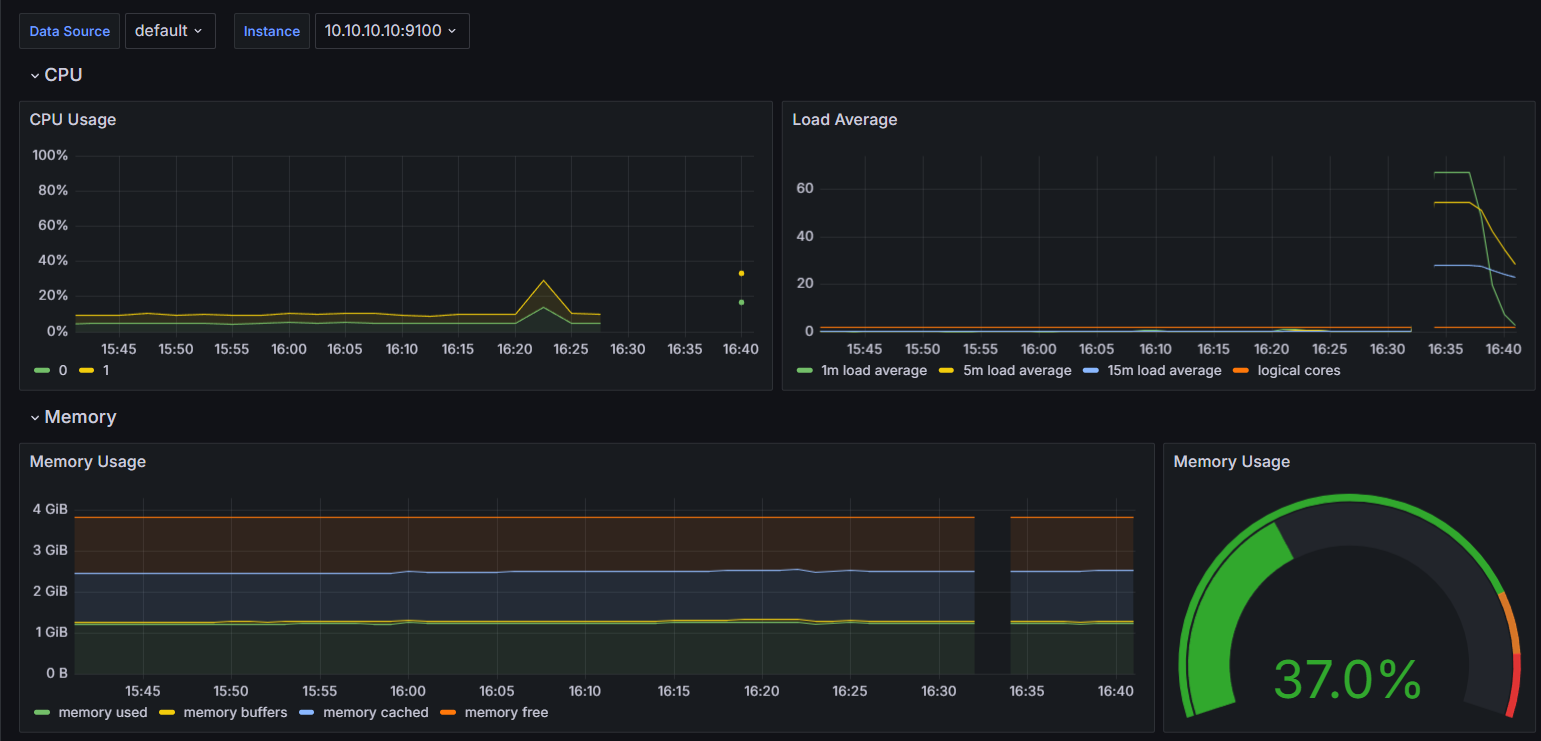
\includegraphics[width=0.9\textwidth]{Images/TC05.png}
    \caption{TC-05 --- Grafana view of per-NF CPU/RAM for the Open5GS core.}
    \label{fig:tc05}
\end{figure}

\textbf{Result:} 0 Prometheus targets DOWN; Grafana shows per-pod CPU/RAM for
all NFs and per-node metrics for the three nodes; total cluster RAM stays under
the 12~GB budget. The dashboards make the UPF's load and the control NFs'
behaviour visible to an operator. \textbf{PASS.}

\subsection{Summary and discussion}

\begin{table}[H]
\centering
\begin{tabular}{cll}
\toprule
\textbf{TC} & \textbf{What it proves} & \textbf{Status} \\
\midrule
TC-01 & 5G core deploys and NFs register (control plane alive) & \textbf{PASS} \\
TC-02 & UE registers and establishes a PDU session            & \textbf{PASS} \\
TC-03 & Real user data flows through the UPF (user plane)      & \textbf{PASS} \\
TC-04 & Stateless NF autoscales under load                    & \textbf{PASS} \\
TC-05 & The running core is fully observable                  & \textbf{PASS} \\
\bottomrule
\end{tabular}
\caption{Test results --- each maps to a requirement in Table~\ref{tab:requirements}.}
\label{tab:test_results}
\end{table}

Taken together, the five tests show the platform is a genuine NFVI: it does not
merely \emph{run containers}, it satisfies the specific demands of a 5G core ---
a separated user-plane data path (TC-03), elastic control functions (TC-04),
and operator-grade visibility (TC-05) --- demonstrated with a real core, not a
placeholder. The principal caveats are that the UPF uses a kernel data path
(so throughput is environment-bound), MongoDB is non-persistent, and the RAN is
simulated by UERANSIM rather than real radio hardware.
